\documentclass[11pt]{article}

\usepackage{graphicx}
\usepackage{listings}
\usepackage{url}
\usepackage{float} % Add this package for the [H] option
\usepackage{listings}
\usepackage{color}

\definecolor{dkgreen}{rgb}{0,0.6,0}
\definecolor{gray}{rgb}{0.5,0.5,0.5}
\definecolor{mauve}{rgb}{0.58,0,0.82}
\usepackage{minted}

\lstset{frame=tb,
  language=Java,
  aboveskip=3mm,
  belowskip=3mm,
  showstringspaces=false,
  columns=flexible,
  basicstyle={\small\ttfamily},
  numbers=none,
  numberstyle=\tiny\color{gray},
  keywordstyle=\color{blue},
  commentstyle=\color{dkgreen},
  stringstyle=\color{mauve},
  breaklines=true,
  breakatwhitespace=true,
  tabsize=3
}

\begin{document}

\begin{titlepage}
    \begin{center}
        
\includegraphics[scale=0.10]{du.png}\par
        \begin{Huge}
            \textsc{University of Dhaka}\par
        \end{Huge}
        \begin{Large}
            Department of Computer Science and Engineering\par \vspace{1cm}
            CSE-3111 : Computer Networking Lab \\[12pt]   
            Lab Report 6 : Implementation of TCP Reno and New Reno congestion control algorithms and their
performance analysis.
        \end{Large}
    \end{center}     
    \begin{large}
        \textbf{Submitted By:\\[12pt]}
            Name: Md Shamsur Rahman Sami\\[5pt]
            Roll No : 57\\[7pt]
            Name: Md Rakib Hossain\\[5pt]
            Roll No : 55\\[12pt]
        \textbf{Submitted On : \\[12pt]}
            March 16, 2024\\[20pt]
        \textbf{Submitted To :\\[12pt]}
            Dr. Md. Abdur Razzaque\\[12pt]
    \end{large}
\end{titlepage}

\tableofcontents  

\newpage

\section{Introduction}

\subsection{Objective}

The primary objective of this experiment is to implement and evaluate the performance of TCP Reno and New Reno congestion control algorithms in a simulated network environment. Specifically, the experiment aims to:

\begin{enumerate}
    \item Implement TCP Reno and New Reno algorithms using suitable programming languages or network simulation tools.
    \item Analyze the behavior of TCP Reno and New Reno under varying network conditions, including different levels of bandwidth, latency, and packet loss.
    \item Compare the performance of TCP Reno and New Reno in terms of key metrics such as throughput, packet loss rate, and round-trip time (RTT).
    \item Evaluate the advantages and limitations of TCP Reno and New Reno in different network scenarios.
    \item Investigate the impact of network parameters on the performance of TCP Reno and New Reno algorithms.
\end{enumerate}

By achieving these objectives, this experiment seeks to provide insights into the behavior and effectiveness of TCP Reno and New Reno congestion control algorithms, contributing to a better understanding of their practical implications in real-world network environments.






\section{Theory}

\subsection{TCP Congestion Control}

Transmission Control Protocol (TCP) is a widely used transport layer protocol in computer networks. One of the key functions of TCP is congestion control, which aims to prevent network congestion by regulating the rate at which data is sent over the network.

TCP congestion control mechanisms operate based on feedback received from the network. When a sender transmits data, it expects to receive acknowledgments (ACKs) from the receiver indicating successful receipt of the data. If the sender receives ACKs promptly, it assumes that the network is operating normally and gradually increases the transmission rate. However, if the sender detects packet loss or other signs of congestion, it reduces the transmission rate to alleviate congestion and prevent further packet loss.

\subsection{TCP Reno}

TCP Reno is a classic congestion control algorithm widely implemented in TCP implementations. It operates based on a combination of slow start and congestion avoidance mechanisms.

\subsubsection{Slow Start}

In the slow start phase, the sender starts with a conservative transmission rate and gradually increases it as acknowledgments are received. Initially, the sender starts by sending one segment of data. Upon receiving an acknowledgment for this segment, it doubles the transmission rate and sends two segments. This process continues until a congestion event occurs.

\subsubsection{Congestion Avoidance}

Once the sender's congestion window (cwnd) reaches a certain threshold, it switches to the congestion avoidance phase. In this phase, the sender increases the transmission rate more gradually, adding one segment to the congestion window for each round-trip time (RTT). This prevents rapid increases in transmission rate that could lead to congestion.

\subsection{TCP New Reno}

TCP New Reno is an enhancement of TCP Reno that improves its performance in scenarios involving fast retransmit and fast recovery.

\subsubsection{Fast Retransmit}

In TCP New Reno, if the sender receives multiple duplicate ACKs for the same data segment, it assumes that the segment has been lost and performs a fast retransmit. This means that the sender retransmits the missing segment without waiting for a timeout.

\subsubsection{Fast Recovery}

After performing a fast retransmit, TCP New Reno enters the fast recovery phase. During fast recovery, the sender reduces its congestion window to half of its current value and retransmits the missing segment. It then enters a congestion avoidance phase similar to TCP Reno.

These mechanisms allow TCP New Reno to recover from packet loss more efficiently than TCP Reno, leading to improved performance in networks with high packet loss rates.

\section{Methodology}

\subsection{Experimental Setup}

The experiments were conducted using a network simulation environment implemented in Python. The simulation environment consisted of a sender node and a receiver node connected by a simulated network link. The sender node implemented the TCP Reno and TCP New Reno congestion control algorithms, while the receiver node provided feedback to the sender regarding packet loss and acknowledgments.

\subsection{Experimental Procedure}

The experiments were designed to evaluate the performance of TCP Reno and TCP New Reno under varying network conditions. The following steps were followed:

\begin{enumerate}
    \item \textbf{Initialization:} The sender node and receiver node were initialized, and the network link parameters were configured, including bandwidth, delay, and packet loss rate.
    
    \item \textbf{Data Transfer:} A file of predefined size was transferred from the sender to the receiver using TCP Reno and TCP New Reno congestion control algorithms.
    
    \item \textbf{Measurement:} Various performance metrics were measured during the data transfer, including throughput, packet loss rate, round-trip time, and congestion window size.
    
    \item \textbf{Analysis:} The collected data was analyzed to compare the performance of TCP Reno and TCP New Reno under different network conditions. Statistical analysis was performed to identify significant differences between the two algorithms.
\end{enumerate}

\subsection{Experimental Variables}

Several variables were considered during the experiments to assess their impact on the performance of TCP Reno and TCP New Reno. These variables included:

\begin{itemize}
    \item Bandwidth: The available bandwidth of the network link.
    \item Delay: The propagation delay between the sender and receiver nodes.
    \item Packet Loss Rate: The rate at which packets were lost in the network.
    \item File Size: The size of the file transferred during the experiments.
\end{itemize}

\subsection{Data Collection}

During each experiment, data was collected on various performance metrics, including:

\begin{itemize}
    \item Throughput: The rate at which data was successfully transferred over the network link.
    \item Packet Loss Rate: The percentage of packets lost during transmission.
    \item Round-Trip Time (RTT): The time taken for a packet to travel from the sender to the receiver and back.
    \item Congestion Window Size: The size of the congestion window maintained by the sender node.
\end{itemize}






\newpagepage

\section{Experimental Result}

\subsection{Task 1}



    \item \textbf{Implement TCP Congestion Control}

    
    
   


    \begin{figure}[H]
        \centering
        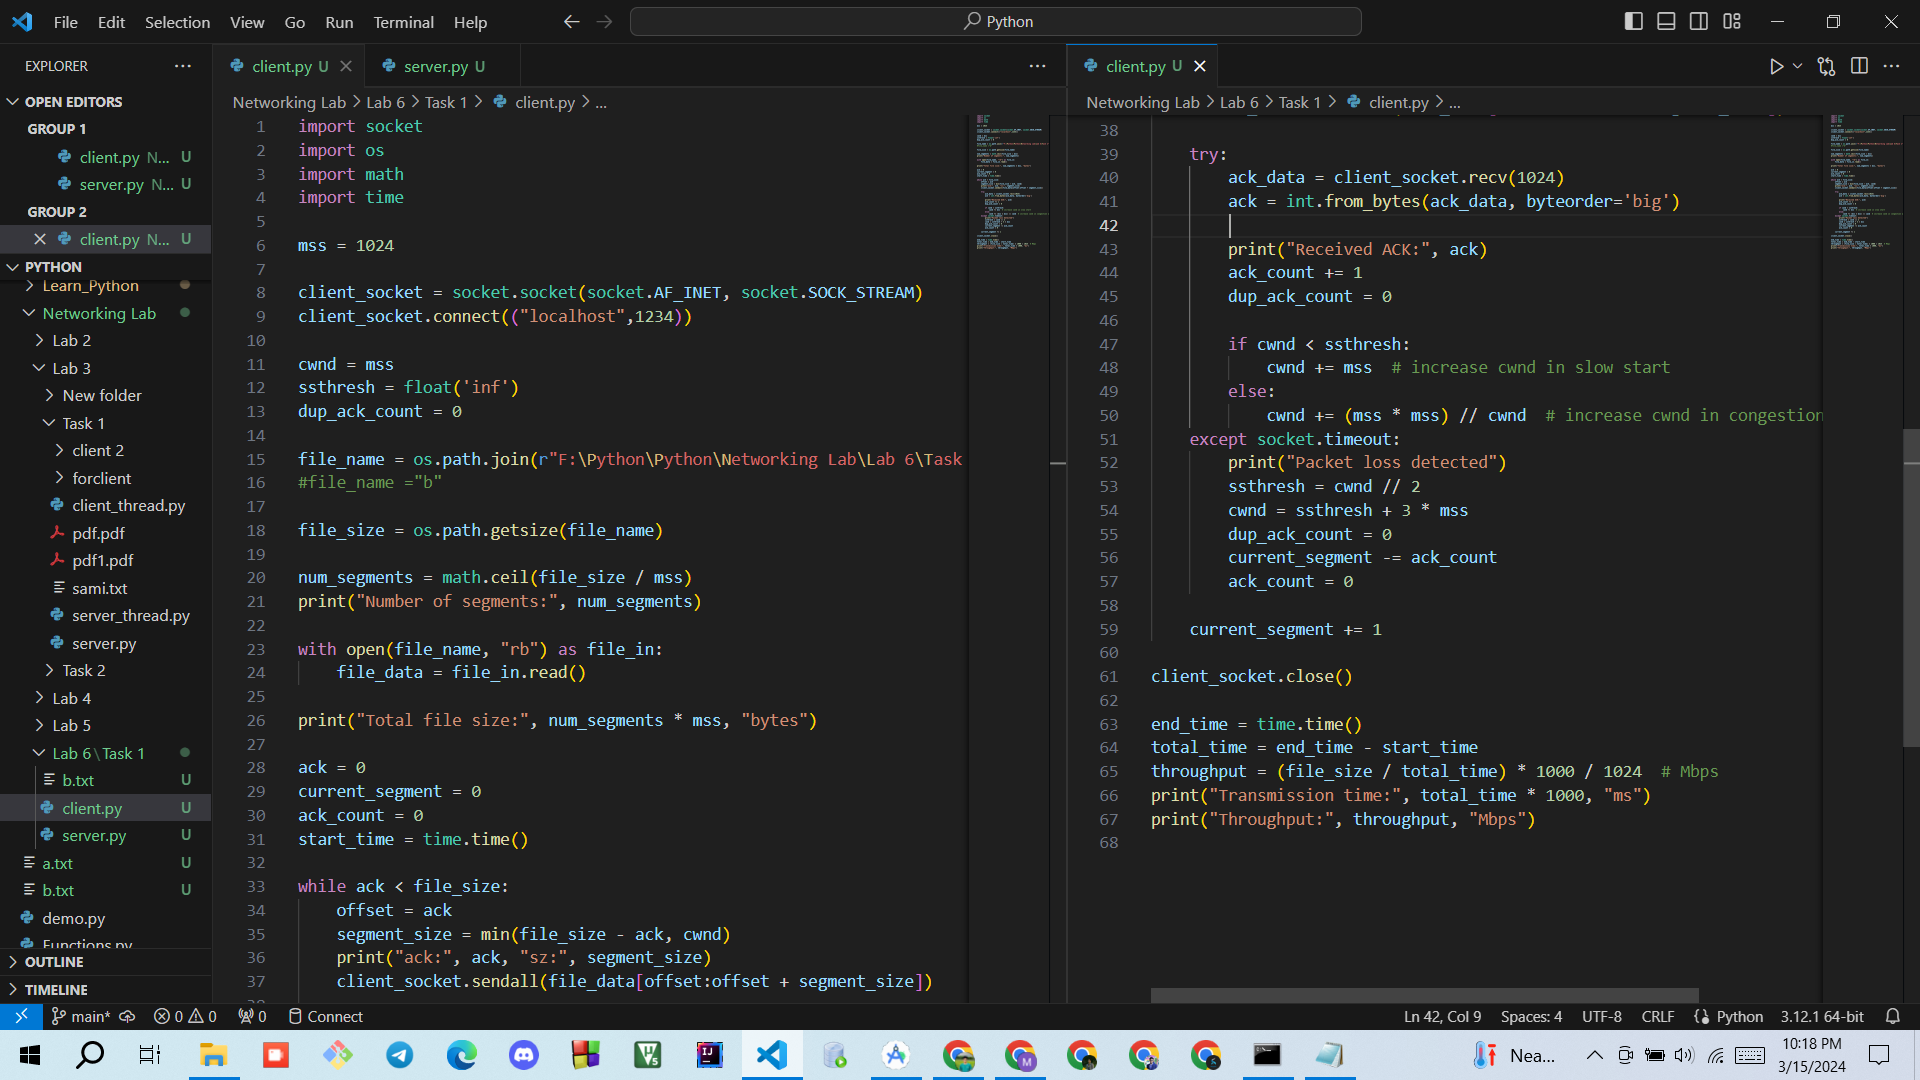
\includegraphics[width=0.8\textwidth]{Screenshot (181).png}
        \caption{Client side code}
        \label{fig:1}
    \end{figure}
    
    \begin{figure}[H]
        \centering
        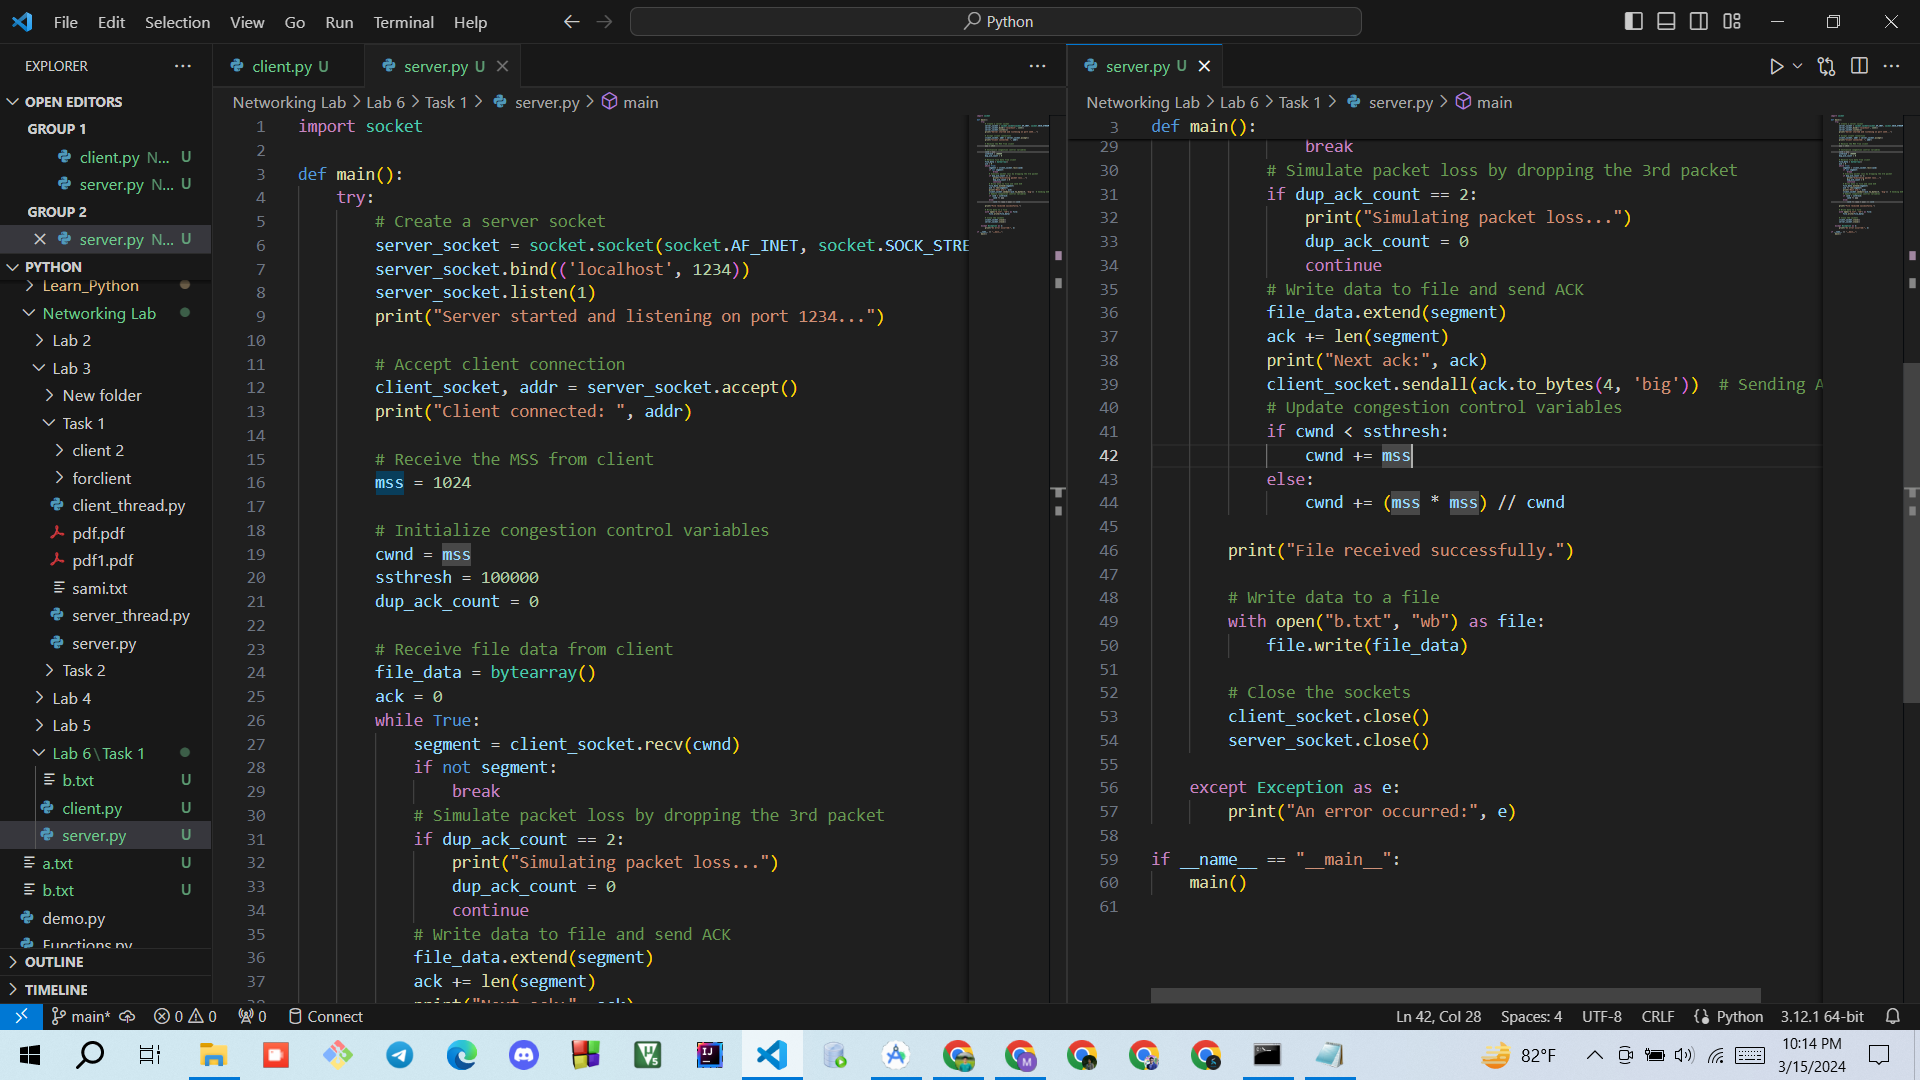
\includegraphics[width=0.8\textwidth]{Screenshot (179).png}
        \caption{Server Side Code}
        \label{fig:2}
    \end{figure}
    \begin{figure}[H]
        \centering
        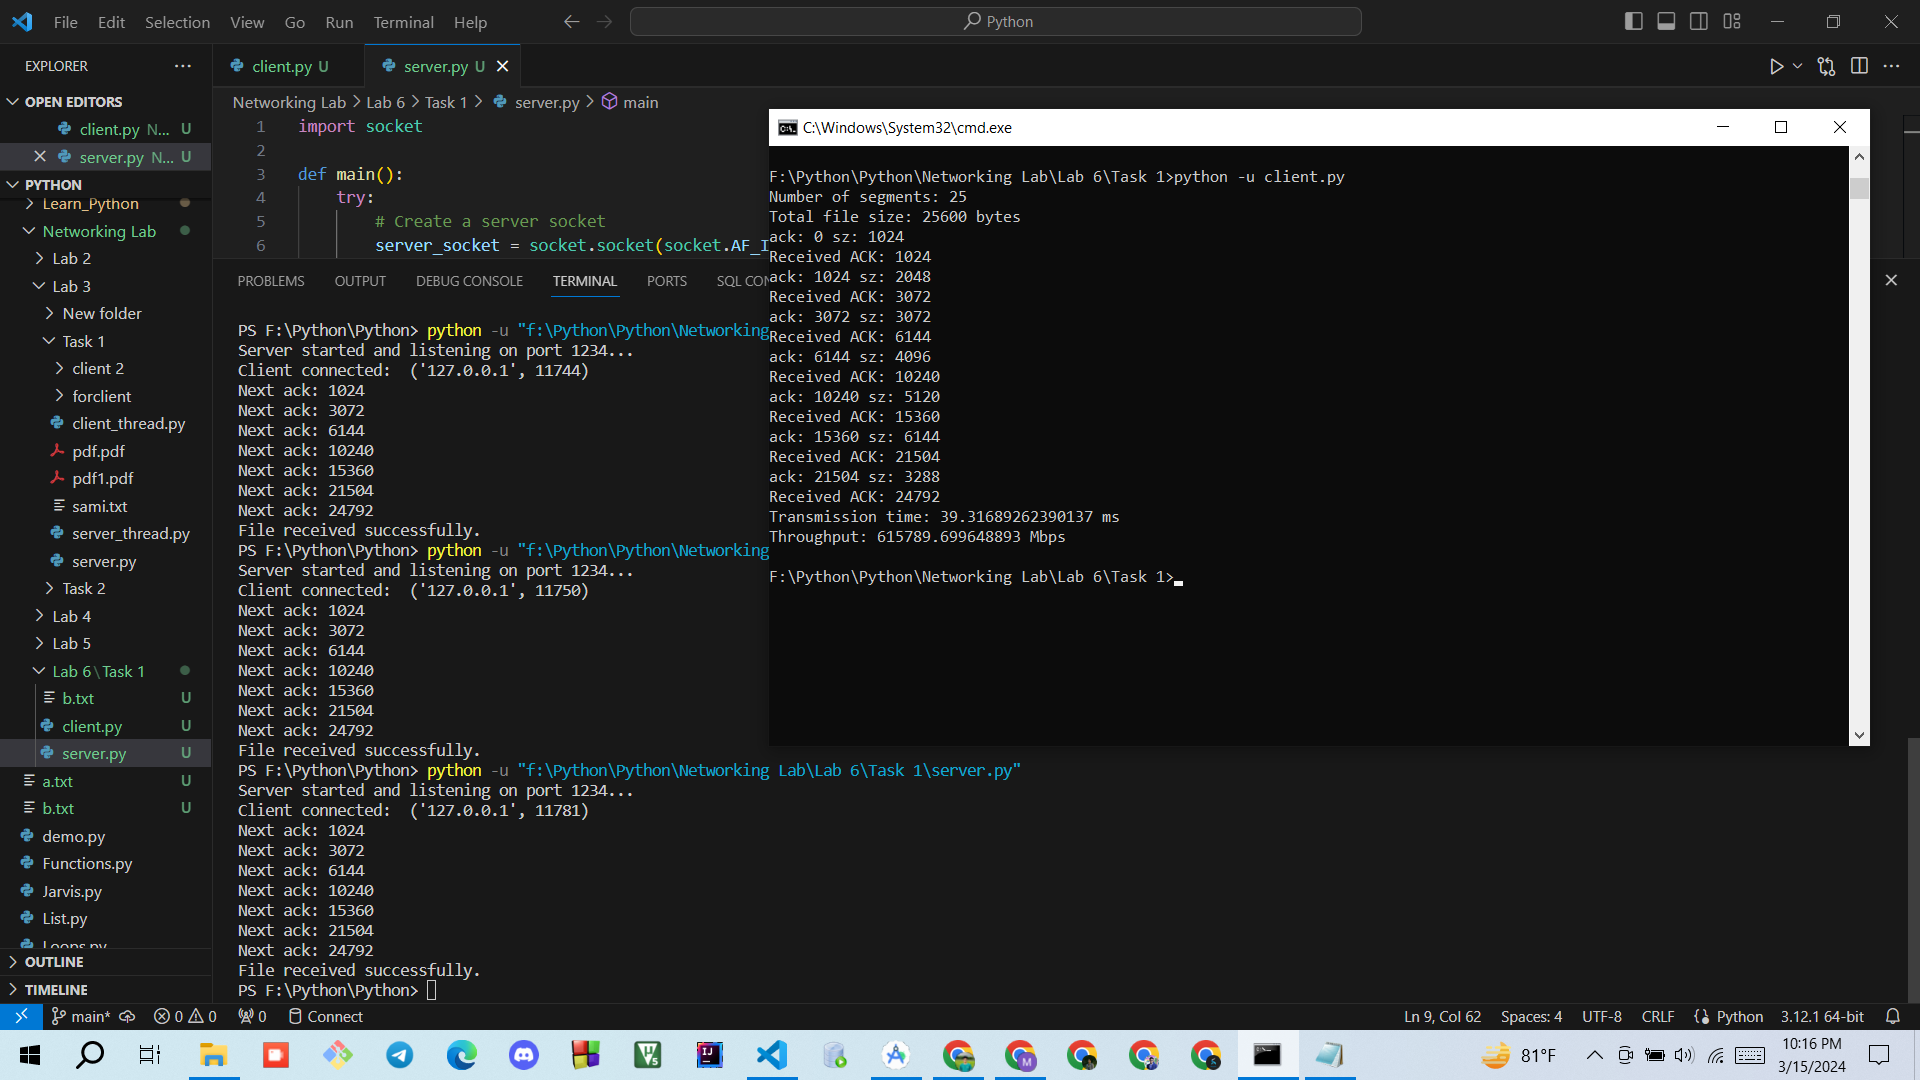
\includegraphics[width=0.8\textwidth]{Screenshot (180).png}
        \caption{Result}
        \label{fig:2}
    \end{figure}
    
    


 

\section{Experience}

\begin{enumerate}
    \item Set up TCP communication between clients and a server.
    \item Implemented TCP congestion control algorithms.
    \item Faced challenges such as packet loss and network optimization.
    \item Troubleshot synchronization issues between components.
    \item Gained insights into TCP congestion control and its impact on network performance.
\end{enumerate}







\begin{thebibliography}{1}
  %\bibitem{book} Computer networking: a top-down approach 6th ed.
  \bibitem{Flow Control and Congestion Control} Flow Control and Congestion Control :\url{https://www.geeksforgeeks.org/difference-between-flow-control-and-congestion-control/}
  \bibitem{Difference} TCP Tahoe and TCP Reno :\url{https://www.geeksforgeeks.org/tcp-tahoe-and-tcp-reno/}
  
  \bibitem{youtube} Youtube: \url{https://youtube.com/watch?v=M6pG9sEVTkg}
 
  

 
\end{thebibliography}



\end{document}

